% =====================================================================
%  IEEE Access submission — LaTeX source
%
%  IMPORTANT: This file uses \documentclass{ieeeaccess}. To COMPILE it you
%  must obtain the class file `ieeeaccess.cls` (plus its bundled .bst) from
%  the IEEE Author Center template pack:
%      https://template-selector.ieee.org/  ->  "IEEE Access"
%  or from the Overleaf "IEEE Access" template gallery entry. Place
%  ieeeaccess.cls (and ieeeaccess.bst / the IEEEtran BibTeX style) in this
%  directory. This .tex is written to be drop-in compatible with that template.
%
%  Build:  pdflatex paper  ->  bibtex paper  ->  pdflatex paper  ->  pdflatex paper
%
%  FORMATTING-ONLY CONVERSION of docs/paper/paper_full_draft.md.
%  No claim, number, or framing was altered. The two positioning-table cells
%  that were previously unresolved (HalluCXR / Zhao "uses report corpus?") have
%  since been filled from the primary sources; see the "% Source:" comments on
%  those rows. Remaining human TODOs are the author/history/funding/biography
%  placeholders (search for "TODO").
% =====================================================================
\documentclass{ieeeaccess}

\usepackage{graphicx}
\usepackage{amsmath}
\usepackage{textcomp}
\usepackage{booktabs}
\usepackage{array}

% arrow shorthand used in a few tables/inline expressions
\newcommand{\arw}{$\rightarrow$}

\begin{document}

\history{Date of current version [DATE — TODO].}
\doi{10.1109/ACCESS.XXXX.DOI}

\title{Auditing Chest X-ray Classifiers for Spurious Shortcuts: Where Blind VLM Naming Succeeds, Where It Fabricates, and What Survives the Failure}

% -----------------------------------------------------------------
% Author block: placeholder only. Do NOT substitute a real person or
% institution without the author's confirmation.
% -----------------------------------------------------------------
\author{[AUTHOR --- TODO]\authorrefmark{1}}
\address[1]{[AFFILIATION / DEPARTMENT --- TODO], [CITY, COUNTRY --- TODO] (e-mail: [EMAIL --- TODO])}

\tfootnote{[FUNDING / ACKNOWLEDGEMENT --- TODO: none asserted by the source draft.]}

\markboth{[AUTHOR --- TODO]: Auditing Chest X-ray Classifiers for Spurious Shortcuts}
{[AUTHOR --- TODO]: Auditing Chest X-ray Classifiers for Spurious Shortcuts}

\corresp{Corresponding author: [AUTHOR --- TODO] (e-mail: [EMAIL --- TODO]).}

\begin{abstract}
Deep chest X-ray classifiers routinely reach high in-distribution accuracy while relying on spurious shortcuts --- features correlated with the label in training but not causally tied to the pathology --- and fail silently when that correlation breaks at a new site. We build an \emph{auditor} that runs a four-stage loop over a pneumothorax classifier: \textbf{detect} that accuracy depends on a confound, \textbf{localize} the confound by attribution, \textbf{name} it in clinical language using a general-purpose vision-language model (VLM) that is never told what to look for, and \textbf{mitigate} the reliance by last-layer retraining. The study is executed as six validation-gated spikes, each with a pre-registered pass/fail threshold and a stop-and-report point.

Detection and localization transfer cleanly from a synthetic confound to a real device confound: we induce a measurable reliance gap (44 percentage points synthetic; 28.75 points on real chest tubes) and localize it (Grad-CAM peak-in-region 100\% synthetic; side-consistency 96.6\% real). Blind VLM naming, however, does not transfer. It passes at near-ceiling on the synthetic marker (precision 0.978, recall 0.90, control-hallucination 0.02) but \textbf{fails on the real chest tube by fabrication}: on tube-free control crops the VLM invents devices --- endotracheal tubes, central lines, catheters --- at a rate of 0.55 (Llama-4-Scout) and 0.83 (Pixtral-12B) in the multi-VLM replication. This cross-model fabrication is the honest negative result at the center of the paper: an auditor built on off-the-shelf general VLMs would raise a fabricated shortcut alarm on a majority of clean images, which is exactly the false-alarm failure the design's precision-over-recall gate was built to catch. What survives the naming failure is mitigation, which never depended on the VLM: Deep Feature Reweighting moves worst-group (pneumothorax-without-tube) accuracy from 0.67 to 0.79 as a 3-seed mean while preserving in-distribution accuracy, using no target-distribution labels. Finally, a real US-to-Spain cross-site AUC drop of 0.192 (95\% CI [0.159, 0.225], bootstrap) exists, but a zero-shot, label-free test of whether reducing the known source shortcut narrows it returns a point estimate indistinguishable from zero ($+0.005$, 95\% CI [$-0.018$, $+0.028$]) --- underpowered to rule out a small-to-moderate effect but not evidence of a real recovery either; the drop is distribution shift this design cannot attribute to the shortcut. We report the naming failure as a headline rather than a footnote, and we report two interpretive claims we withdrew after running their falsifying controls.
\end{abstract}

\begin{IEEEkeywords}
Chest X-ray, deep feature reweighting, distribution shift, hallucination, medical imaging, model auditing, shortcut learning, spurious correlation, vision-language models, worst-group accuracy.
\end{IEEEkeywords}

\titlepgskip=-21pt
\maketitle

% =====================================================================
\section{Introduction}
\IEEEPARstart{D}{eep} chest X-ray (CXR) classifiers can reach high in-distribution accuracy while keying on features that are correlated with the label in the training data but not causally related to the pathology --- scanner text, laterality and positioning markers, hospital- or device-specific artifacts. Zech et al.\ \cite{zech2018} showed that CNNs generalize worse across hospitals than within them and can identify the source hospital system with $\sim$99.95--99.98\% accuracy; DeGrave, Janizek \& Lee \cite{degrave2021} showed COVID-19 CXR models keying on text markers and patient positioning rather than pathology. Such models appear accurate and fail under distribution shift, which is a patient-safety problem: a model that keys on the chest tube used to \emph{treat} a pneumothorax rather than on the pneumothorax itself will silently mispredict exactly on the untreated patients where correct detection matters most.

Auditing a classifier for this failure has four parts: (1) \textbf{detect} that it relies on a shortcut, (2) \textbf{name} the shortcut in clinical terms without being told what to look for, (3) \textbf{mitigate} the reliance, and (4) \textbf{prove recovery} under out-of-distribution shift. Prior work tends to address only some. Shortcut-diagnosis papers (Zech \cite{zech2018}; DeGrave \cite{degrave2021}; Jim\'enez-S\'anchez et al.\ \cite{jimenez2023}) detect shortcuts by expert or statistical analysis but do not automate the naming step. Generative-correction methods such as RoentMod \cite{roentmod} edit images with a diffusion pipeline to correct shortcuts, at the cost of a heavy generative apparatus and fine-tuning. Worst-group robustness methods (GroupDRO \cite{sagawa2020groupdro}, JTT \cite{liu2021jtt}, DFR \cite{kirichenko2022dfr}) mitigate but assume the groups are already known. The nearest label-free naming prior art, LADDER \cite{ladder}, names a classifier's shortcut with a foundation model in radiology, but routes the image through a captioner plus a text-only LLM and evaluates discovery only through downstream mitigation accuracy --- with no false-alarm gate.

\textbf{The gap this paper targets} is prompt-free, generative-model-free naming, wired into a full detect\arw{}localize\arw{}name\arw{}mitigate loop and scored directly against ground truth under a \emph{control-hallucination gate}: the rate at which the auditor names a device on a confound-free image. That gate is the design's identity. For an auditor, a fabricated confound costs more than a missed one, because a tool that invents shortcuts is worse than no tool; so precision is gated above recall, and the fabrication rate on clean images is a pass/fail condition on the capability itself, measured separately.

\textbf{Contributions.}
\begin{itemize}
\item A validation-gated auditor loop that detects, localizes, and mitigates a real device shortcut in a pneumothorax classifier with no target-distribution labels, built on a confound-agnostic core that serves synthetic, real-device, and cross-site settings from one implementation.
\item The paper's central finding, reported honestly as a negative result: blind, general-purpose VLM naming \textbf{succeeds on a synthetic confound and fails on a real device confound by fabrication}, and the failure is a cross-model property (Llama-4-Scout and Pixtral-12B both fabricate devices on a majority of clean crops), independently corroborated by HalluCXR \cite{hallucxr}.
\item Mechanism experiments that bound \emph{why} naming breaks: fabrication is not driven by the confound's visibility (a recall cliff, not a hallucination cliff), and it is grounded in the image rather than blind recitation --- it is prior-driven over-reading of an ambiguous salient region.
\item A zero-shot, label-free source-side test of whether a known shortcut explains a measured cross-site generalization gap, reporting a null result: the 0.192 US-to-Spain drop is distribution shift not shown to be shortcut-driven.
\item An account of two interpretive claims withdrawn after running the specific controls that falsified them, treated as a first-class result rather than hidden.
\end{itemize}

% =====================================================================
\section{Related Work}
\textbf{Shortcut learning in chest radiography} is well established. Zech et al.\ \cite{zech2018} showed CNNs generalize worse across hospitals than within them, and can identify the hospital system with $\sim$99.95--99.98\% accuracy. DeGrave, Janizek \& Lee \cite{degrave2021} showed COVID-19 CXR models keyed on text markers and patient positioning rather than pathology. Jim\'enez-S\'anchez, Juodelyte, Chamberlain \& Cheplygina \cite{jimenez2023} present a manual and statistical shortcut-detection case study on chest X-rays. These works establish that shortcuts exist and are dangerous, and diagnose them by expert analysis or statistical association; none automates the \emph{naming} step through a general-purpose model.

\textbf{Correcting shortcuts generatively.} RoentMod (arXiv:2509.08640) \cite{roentmod} pairs a medical image generator (RoentGen) with an image-to-image editor to produce counterfactual CXRs with specified findings while preserving anatomy, reporting discrimination improvements of 3--19\% AUC internally and 1--11\% externally, with 93\% of generated images rated realistic by readers. It is the closest correction-side prior art and the method we most directly contrast against: it relies on a generative diffusion pipeline and fine-tuning, where our naming step uses one free API pass over $\sim$200 crops with no generative model at all. That is a genuine trade rather than a strict improvement --- RoentMod's correction-only design never had to clear the bar our naming step failed.

\textbf{Mitigation baselines.} GroupDRO (Sagawa et al., 2020) \cite{sagawa2020groupdro} optimizes worst-group loss but requires group labels; JTT (Liu et al., 2021) \cite{liu2021jtt} upweights an ERM model's errors to approximate group robustness without them; DFR (Kirichenko et al., 2022) \cite{kirichenko2022dfr} retrains only the last layer on group-balanced data, reaching 92.9\% worst-group on Waterbirds and 70.1\% on CivilComments at a fraction of GroupDRO's cost, on the premise that the backbone already encodes core features. Follow-up work (arXiv:2308.00473) \cite{dfr_followup} questions whether last-layer retraining always suffices --- a caution our synthetic-tag results directly corroborate, since on a \emph{pure}-shortcut backbone DFR's in-distribution recovery is incomplete. These methods assume the groups are already known; our loop attempts to discover and name the confound first.

\textbf{Concurrent work on the same shortcut.} Zhao et al.\ (arXiv:2604.17110) \cite{zhao2026} use an autonomous LLM coding-agent pipeline that, among other tasks, reduces chest-drain reliance for pneumothorax classification on NIH-derived data, reporting 60\%\arw{}31\% and 50\%\arw{}18\% reliance reduction on two datasets. Same target shortcut, different mechanism (agentic pipeline search vs.\ last-layer retraining), different metric (\% reliance vs.\ worst-group accuracy and reliance gap). It reports no VLM-naming step, no control-hallucination measurement, and no cross-site transfer test. We read it as independent, contemporaneous confirmation that this real shortcut is a live target reached by a different route --- corroborating, not competing.

\textbf{Foundation-model shortcut auditing (closest analogues to the naming step).} LADDER (Ghosh et al., Findings of ACL 2025) \cite{ladder} is the nearest medical-imaging prior art: it uses an LLM's latent domain knowledge to hypothesize a classifier's biases without pre-specified attribute labels, and evaluates partly on chest X-rays. Three differences make it a neighbor rather than the same method: (i) it reads the image as \emph{text} (BLIP/GPT-4o captions plus activation-to-text projection), reasoning with a text-only LLM, where we feed the Grad-CAM crop \textbf{pixels} to a general VLM with no captioner and no report corpus; (ii) it scores discovery via slice Precision@10 and downstream worst-group accuracy, with \textbf{no control-hallucination gate}; (iii) its discovery is in service of mitigation, so a naming failure like our V4b would be absorbed into a mitigation score rather than surfaced. SpurLens (arXiv:2503.08884) \cite{spurlens} uses GPT-4 plus open-set detectors to discover spurious cues multimodal LLMs over-rely on in natural images, and measures hallucination amplification (objects hallucinated up to 10$\times$ more often when a spurious cue is present). RaVL (arXiv:2411.04097) \cite{ravl} discovers region-level spurious correlations inside a fine-tuned VLM's own errors and mitigates with a region-aware loss ($+8.2\%$ worst-group accuracy; 191\% discovery improvement, across 654 VLMs). Both are close mechanism analogues but neither touches medical imaging, blind clinical naming, or a control-hallucination-gated metric. MIMM-X (arXiv:2511.22990) \cite{mimmx} disentangles a \textbf{pre-specified} confounder via mutual-information objectives --- the opposite of a blind design, and evidence that the standard alternative still assumes foreknowledge of the confound. Grad-CAM-style attribution (Selvaraju et al.) \cite{gradcam} localizes \emph{where} a model looks --- our localization step uses it --- but does not name what it found.

\textbf{VLM reliability on chest radiographs} bears directly on our naming result. HalluCXR (arXiv:2605.20469) \cite{hallucxr} benchmarks 6 VLMs on 856 chest radiographs, finding 61.9--82.3\% overall and 36.4--80.2\% ``clinically dangerous'' hallucination rates, with severity highest on normal images (51.9\% severity-3 on normals). This corroborates our 0.50--0.83 control-hallucination on clean crops in a different model population on a different task (diagnostic findings vs.\ device naming). Lotfinia et al.\ (arXiv:2606.17710) \cite{lotfinia2026} show VLMs can answer CXR questions from language priors without attending to the image --- the direct threat to our naming step's interpretation, which our Experiment 2 addresses and does not support as an explanation of the failure (Section~\ref{sec:mechanism}). Specialist CXR-VLMs (CXR-LLaVA, arXiv:2310.18341 \cite{cxrllava}; LLaVA-Rad \cite{llavarad}) are fine-tuned on radiology data; we deliberately used a general-purpose, non-fine-tuned model to test the lower-barrier claim.

\textbf{Ground-truth dependency.} NEATX (Cheplygina et al., arXiv:2309.02244) \cite{neatx} supplies the non-expert chest-drain annotations our real-confound experiments rely on. This is a data dependency, credited distinctly from prior art.

\subsection{Positioning}
Table~\ref{tab:positioning} places this work against the closest analogues. The nearest prior art, LADDER \cite{ladder}, shares our premise --- name a classifier's shortcut with a foundation model, in radiology, without attribute labels --- but reads the image as text and evaluates discovery only through the downstream accuracy of the mitigation it enables. Our method reads the classifier's saliency region as pixels, through a blind-prompted general VLM, and evaluates the name directly against ground truth under a control-hallucination gate. That gate is what converts ``the VLM produced a plausible shortcut description'' into a testable claim, and it is why we can report --- rather than absorb into a mitigation score --- that blind naming \emph{fails} on a real device confound while succeeding on a synthetic one. What appears genuinely novel after an exhaustive July-2026 search: no paper (a) performs blind general-VLM naming of a CXR shortcut scored on precision/recall/control-hallucination, or (b) runs a zero-shot, label-free source-side intervention to test whether a known shortcut explains a cross-site gap, reporting the null honestly.

\begin{table*}[!t]
\caption{Positioning against the closest analogues. Two cells remain genuinely unresolved in our source documents and are flagged as visible TODO comments in the source, not invented.}
\label{tab:positioning}
\centering
\footnotesize
\renewcommand{\arraystretch}{1.3}
\begin{tabular}{p{2.3cm} p{2.6cm} p{2.3cm} p{3.0cm} p{3.4cm}}
\toprule
\textbf{method} & \textbf{data modality} & \textbf{uses report corpus?} & \textbf{control-hallucination gate?} & \textbf{models tested} \\
\midrule
\textbf{This work (auditor)} & chest X-ray (NIH, PadChest); NEATX device labels & \textbf{No} --- blind prompt on saliency crops only & \textbf{Yes} --- separate gate at $<$10\% on confound-free controls; the gate that failed V4b & 2 general-purpose (Llama-4-Scout, Pixtral-12B) + specialist/scale arm (CheXagent-2-3B \& -8B, qwen2.5-vl-7b) --- over-name vs under-name axis \\
\textbf{LADDER} (Ghosh et al., Findings of ACL 2025) & image $\rightarrow$ \textbf{caption} (BLIP/GPT-4o) + activation-to-text & \textbf{Yes} --- captioner required & \textbf{No} --- worst-group accuracy + slice Precision@10 & reasoning LLMs (GPT-4o, Claude, Gemini, LLaMA); classifiers on NIH-CXR, RSNA, VinDr, Waterbirds, CelebA, MetaShift \\
\textbf{HalluCXR} (arXiv:2605.20469) & chest X-ray (856 radiographs) & \textbf{Yes} --- radiologist reports supplement CheXpert labels as ground truth & No --- it \emph{measures} hallucination as the object of study (61.9--82.3\% overall; severity highest on normals) & 6 VLMs: BiomedCLIP, Gemini 3 Flash, GPT-5.1, InternVL2, LLaVA-NeXT-Mistral, Qwen2-VL \\
% Source: arXiv:2605.20469v1 full text --- models section; ground truth uses original radiologist reports supplementing CheXpert labels.
\textbf{Zhao et al.} (arXiv:2604.17110) & chest X-ray (NIH-derived) & \textbf{No} --- clinician plain-language description, not report text & \textbf{No} --- reports \% reliance reduction (60\%$\rightarrow$31\%, 50\%$\rightarrow$18\%); no naming step to gate & LLM coding-agent pipeline; no VLM-naming arm \\
% Source: arXiv:2604.17110 abstract --- takes a clinician's plain-language description; no report corpus.
\bottomrule
\end{tabular}
\end{table*}

% =====================================================================
\section{Methods}
\subsection{Overview}
We audit a chest X-ray classifier for reliance on spurious shortcuts through a four-stage loop: \textbf{detect} that the classifier's accuracy depends on a confound, \textbf{localize} the confound via attribution, \textbf{name} it in clinical language using a general-purpose vision-language model (VLM) that is never told what to look for, and \textbf{mitigate} the reliance by last-layer retraining. The loop is evaluated on a synthetic confound, a real device confound, and a real second site. The study was executed as six validation-gated spikes (V1--V6), each with a pre-registered pass/fail threshold and a stop-and-report point, so that a failed stage terminates a claim rather than being iterated around.

Architecturally, this discipline produced a \textbf{confound-agnostic core}: the attribution (Grad-CAM) and mitigation (DFR) machinery take a generic confound description --- a region box, or a \texttt{(confound, label)} column pair --- so the same modules serve the synthetic tag, the real chest tube, and the cross-site case without modification. The one component with an external, rate-limited dependency --- the VLM-naming step --- is isolated behind a \texttt{crops/ + manifest.json} $\rightarrow$ \texttt{predictions.jsonl} file contract, so the provider is interchangeable and no downstream computation depends on it. No method in the mitigation path imports the naming module, enforcing by construction that the mitigation result cannot depend on the VLM.

\subsection{Data and Model}
The primary corpus is NIH ChestX-ray14 (112,120 images, resized to 224$\times$224), with patient-disjoint train/validation/test splits (73k/13k/25.6k) built from the official split lists; image-level splitting is never used, as it leaks a patient's other studies across splits. The target pathology is pneumothorax (roughly 3--5\% prevalence depending on split). The classifier is an ImageNet-pretrained DenseNet-121 trained with automatic mixed precision, batch size 16, and a \texttt{pos\_weight}-corrected binary cross-entropy loss for the class imbalance.

Real chest-drain ground truth comes from \textbf{NEATX} (Cheplygina et al., arXiv:2309.02244) \cite{neatx}, which supplies non-expert chest-drain annotations for a subset of ChestX-ray14 and PadChest. The second site is \textbf{PadChest} (Hospital San Juan, Spain), used in its 224$\times$224 release; a 7,572-image working subset (573 pneumothorax-positive, 7,000 negative) was extracted under a disk constraint.

\subsection{V1 --- Pipeline Sanity}
A baseline pneumothorax classifier is trained end-to-end and gated on in-distribution test AUC $\geq 0.75$. This spike exists solely to establish that any subsequent degradation is attributable to an intervention rather than to a broken pipeline.

\subsection{V2 --- Shortcut Induction}
A synthetic confound --- a 20$\times$20 opaque corner tag --- is stamped onto training images with correlation strength \emph{p} to the pneumothorax label. Reliance is quantified as the \textbf{reliance gap}: accuracy with the confound aligned as trained, minus accuracy with the confound removed, measured on a class-balanced subset. A third condition (tag \emph{flipped}, i.e.\ anti-correlated) provides a lower bound. The gate is a gap $>$ 20 percentage points. A companion \textbf{correlation-strength sweep} trains the same architecture at \emph{p} in $\{0.6, 0.7, 0.8, 0.9, 0.95\}$ to characterize how reliance and its mitigability scale with confound strength.

\subsection{V3 --- Attribution Localizes the Confound}
Grad-CAM is computed on the shortcut-reliant checkpoint. Localization is scored with a pointing game (\texttt{peak\_in\_region}) against a generic box $(y_0, x_0, y_1, x_1)$, plus a \texttt{mass\_fraction} statistic. Crucially, the same images with the confound \emph{removed} serve as a control, which rules out ``that corner is always salient'' as an alternative explanation. All attribution geometry is confound-agnostic: no function knows whether the box contains a synthetic tag or a real device, so the identical code serves the synthetic and real settings.

\subsection{V4 --- Blind VLM Naming}
Salient crops from confound-positive images, plus confound-free control crops, are exported with a manifest carrying exact \texttt{has\_confound} labels the VLM never sees. Crops are captioned by a general-purpose, non-fine-tuned VLM under a \textbf{blind prompt} that never mentions the target (``describe anything artificial, non-anatomical, or out of place\ldots if normal, say so''). Free-text descriptions are scored by conservative keyword matchers --- \texttt{names\_confound} for the synthetic-marker vocabulary, \texttt{names\_tube} for device-specific vocabulary (tube / drain / catheter / line / wire) --- into precision, recall, and \textbf{control-hallucination}: the rate at which a device or marker is named on a confound-free crop. Matchers are unit-tested not to fire on generic anatomy language.

The naming stage is deliberately split into two gates with different bars, because they test different things:
\begin{itemize}
\item \textbf{V4a (synthetic tag)} proves the \emph{method} works where ground truth is exact and the confound is unambiguous. Gate: precision $\geq 0.90$, recall $\geq 0.90$, control-hallucination $<$ 10\%.
\item \textbf{V4b (real chest tube)} proves the method \emph{transfers}. Gate: precision $\geq 0.80$, recall $\geq 0.70$, control-hallucination $<$ 10\%.
\end{itemize}

Precision is gated above recall by design: for an auditor, a fabricated confound costs more than a missed one, since a tool that invents shortcuts is worse than no tool. The control-hallucination bar is measured separately and is the hardest to relax. The original design specified a six-model roster (Llama-4-Scout, Llama-4-Maverick, Gemini, GPT-4o, Pixtral-12B, and the specialist arm reported separately in Section~\ref{sec:specialist}); two of those six did not reach a result before the run: Maverick was retired by its provider (Groq) before it could be run, and GPT-4o was excluded for lack of a provisioned API token --- both practical access constraints on a zero-budget project, not results. Two general-purpose VLMs were run through the identical pipeline on the identical crops: \textbf{Llama-4-Scout} and \textbf{Pixtral-12B}. A third (Gemini) was not run to completion because its free tier caps daily requests per model below the 200 crops required; it is not reported as a result.

\subsection{V5 --- Mitigation}
Mitigation is \textbf{Deep Feature Reweighting (DFR)}: extract frozen penultimate features, draw a group-balanced sample over \texttt{(confound, label)} groups, fit a logistic head on standardized features, and swap only the final linear layer. Group balancing handles the structurally empty group (chest tubes co-occur almost exclusively with pneumothorax-positives, so \texttt{(tube=1, label=0)} does not exist). \textbf{ERM} and \textbf{JTT} (upweighting the frozen model's own errors and refitting the head) are run from the same feature-extraction path as baselines, over 3 seeds. Because none of these three methods import the naming module, this comparison doubles as the \textbf{naming-off ablation}: the loop's mitigation result cannot depend on the VLM. Metrics are worst-group accuracy (pneumothorax \emph{without} the confound), in-distribution accuracy (pneumothorax \emph{with} the confound), and the reliance gap.

A \textbf{linear probe} control freezes a shortcut-trained backbone and fits a fresh head on confound-free images, to test directly whether shortcut reliance hollows out or merely degrades core-feature learning.

\subsection{V6 --- Cross-Site Generalization}
The V1 model is evaluated unchanged on PadChest. Two mitigation variants are distinguished, and the distinction is the point of the spike:
\begin{itemize}
\item \textbf{Supervised target adaptation} --- fit the last layer on \emph{labeled} PadChest data. This tests adaptation, not shortcut mitigation: it would help even with no shortcut present.
\item \textbf{Zero-shot source-DFR} --- reduce the known source-side shortcut using NIH data only, touch \textbf{no} target labels, then evaluate PadChest. This is the test that can license a claim that the cross-site gap is shortcut-driven.
\end{itemize}

PadChest images are 16-bit while NIH images are 8-bit. Reconciling this at load time (rather than by changing the model's evaluation transform) is required for validity; the NIH reference AUC is re-measured after every such change and serves as the control that validates any cross-site number.

\subsection{Reproducibility}
Every run is config-driven (typed YAML with inheritance and CLI overrides), fixed-seeded, and logged to a timestamped directory containing the resolved config, \texttt{metrics.json}, and a checkpoint. Dataset paths are configuration values; no image or checkpoint is version controlled. The codebase is organized into confound-agnostic modules (\texttt{data/}, \texttt{train/}, \texttt{shortcut/}, \texttt{attribution/}, \texttt{discovery/}, \texttt{evaluation/}, \texttt{mitigation/}, \texttt{report/}) with 128 passing tests concentrated on the parts most likely to silently break: patient-disjointness of the loaders, the naming scorer's matchers (tested \emph{not} to fire on generic anatomy), and the DFR group-balancing.

\textbf{Compute cost.} All local training/evaluation ran on a single consumer GPU (RTX 3050, 6GB); the core reported runs (V1/V2/V3 training and attribution, the 3-seed Phase-3 baseline table, V5, V6) total approximately 2 GPU-hours by \texttt{run.log} timestamp. The naming stage used 5,600 free-tier VLM API calls in total across the canonical V4a/V4b runs and every extension experiment (opacity sweep, occlusion study, multi-VLM and specialist arms); no generative model or fine-tuning step is used anywhere in the pipeline. This is the quantified basis for the compute-efficiency contrast drawn against RoentMod in Related Work --- we report our own cost directly rather than estimate RoentMod's, which is not published in comparable units.

% =====================================================================
\section{Results}
The classifier trains to a sane baseline (V1: test AUC \textbf{0.8448}, validation 0.8269 --- within the published NIH-pneumothorax range) and cheats measurably when given the opportunity (V2: reliance gap \textbf{44pp}; aligned 0.94, removed 0.50, flipped 0.05). The removed-accuracy landing at exactly 0.500 is the pure-shortcut fingerprint, predicted and verified with a synthetic tag-detector before the run rather than rationalized after it. Attribution localizes the confound essentially perfectly (V3: peak-in-box \textbf{100\%} on tagged positives vs \textbf{0.5\%} on the same images untagged; mass fraction 0.14 in a box covering 0.8\% of image area).

\subsection{Naming Succeeds on the Synthetic Confound and Fails on the Real One}
\textbf{V4a passes at near-ceiling.} Blind-prompted Llama-4-Scout named the injected tag with precision \textbf{0.978}, recall \textbf{0.90}, and control-hallucination \textbf{0.02}, over 100 tagged positives and 100 confound-free controls. Recall landed exactly at its 0.90 bar on ten genuine model misses --- an easy target already producing misses, which foreshadowed the harder case. The keyword matcher was corrected mid-analysis after a manual audit of all 23 original misses found that roughly 13 were the VLM correctly describing a ``rectangular / opaque white object'' in phrasing the initial regex did not cover; the fix was verified not to have relaxed the control-hallucination check, which remained at 0.02.

\textbf{V4b fails, and fails specifically on fabrication.} On real chest-tube crops the same model, same prompt, same pipeline yielded precision \textbf{0.57}, recall \textbf{0.66}, control-hallucination \textbf{0.50}. Detection and localization still worked on the real confound (tube reliance gap \textbf{28.75pp}; Grad-CAM side-consistency \textbf{96.6\%}) --- only naming broke. An audit of the control crops found \textbf{47 of 50} false positives explicitly naming a device (``endotracheal tube,'' ``central line,'' ``catheter'') on images containing none: genuine hallucination, not a scorer artifact.

This is the pre-registered pivot condition (V4a passes, V4b fails), and it was executed as specified rather than iterated around: automated naming is withdrawn as a validated capability for real device confounds, and V4b is reported as a bounded negative result.

\begin{figure*}[!t]
\centering
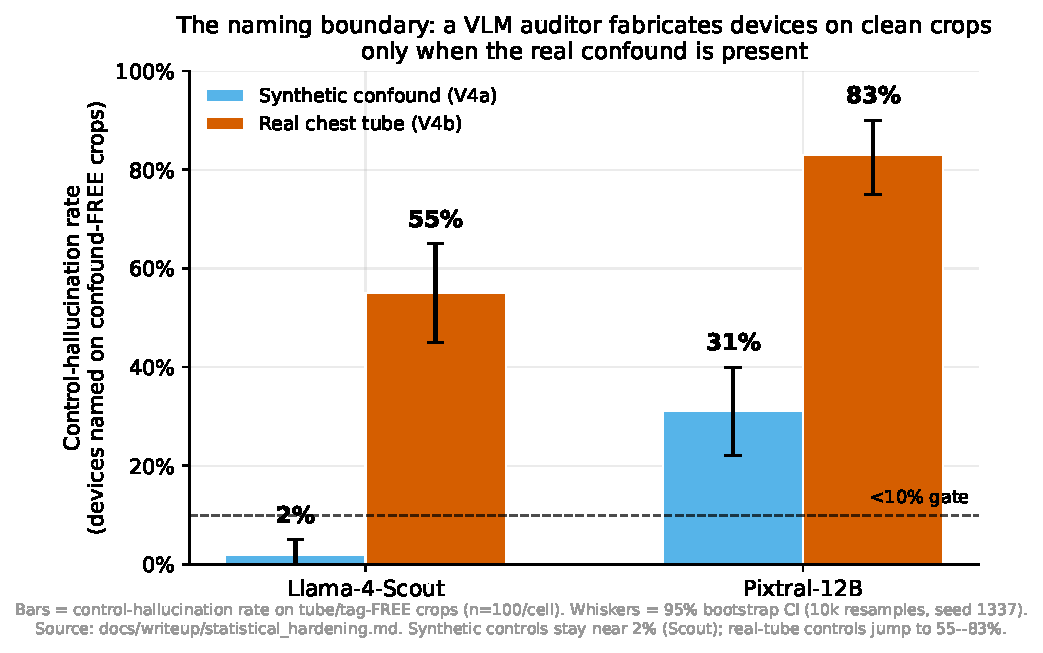
\includegraphics[width=0.9\textwidth]{figures/figure1_naming_boundary.pdf}
\caption{The naming boundary: control-hallucination (device named on a confound-free crop) for each VLM on the synthetic confound versus the real chest tube. The boundary is \textbf{per-model}, not a flat clean split: Llama-4-Scout rises from \textbf{0.02} (synthetic) to \textbf{0.55} (real); Pixtral-12B rises from \textbf{0.31} (synthetic) to \textbf{0.83} (real). Both fabricate a device on a majority of clean control crops in the real-device setting; Pixtral already fabricates on nearly a third of clean synthetic-setting crops. The $<$10\% gate is cleared only by Scout on the synthetic confound.}
\label{fig:naming_boundary}
\end{figure*}

\subsection{The Failure Is a Property of General VLMs, Not of One Model}
The obvious objection to a single-model negative is that a different VLM would not fail. We re-ran the \textbf{identical} 200 V4b crops, the \textbf{identical} blind prompt, and the \textbf{identical} \texttt{names\_tube} matcher through two independent VLM families (Table~\ref{tab:multivlm}).

\begin{table}[!t]
\caption{Multi-VLM replication on the identical V4b crops, prompt, and matcher. Both models fabricate a device on a majority of clean control crops.}
\label{tab:multivlm}
\centering
\begin{tabular}{lccc}
\toprule
\textbf{model} & \textbf{precision} & \textbf{recall} & \textbf{control-hall.} \\
\midrule
Llama-4-Scout & 0.545 & 0.660 & \textbf{0.550} \\
Pixtral-12B & 0.494 & 0.810 & \textbf{0.830} \\
\bottomrule
\end{tabular}
\end{table}

Both fabricate a device on a \emph{majority} of clean control crops. The Scout re-run (0.550) reproduces the original V4b value (0.500) within run-to-run API and decoding drift; Pixtral is markedly worse. Audit of the raw text: Scout invents specific devices on clean anatomy (``endotracheal tube,'' ``central venous catheter''); Pixtral emits near-identical boilerplate (``linear radiopaque object\ldots looks like a medical device or foreign body'') on \textbf{83 of 100} control crops. The matcher is conservative on positives --- it does not fire on hedged ``linear artifact'' phrasing --- which depresses recall in the safe direction rather than inflating hallucination.

An auditor built on off-the-shelf general-purpose VLMs would therefore raise a fabricated shortcut alarm on \textbf{55--83\%} of clean images (Scout 55\%, Pixtral 83\%). This is precisely the false-alarm cost the precision-over-recall gate was designed to catch, now established as a cross-model property. A post-hoc bootstrap (10,000 resamples, seed 1337) confirms the synthetic-vs-real gap is statistically significant for both models: the 95\% CI on the V4a-minus-V4b control-hallucination difference excludes zero (Scout $-0.53$ [$-0.63, -0.43$]; Pixtral $-0.52$ [$-0.64, -0.40$]), and Fisher's exact rejects independence (Scout $p = 1.22\mathrm{e}{-18}$; Pixtral $p = 7.56\mathrm{e}{-14}$). The result is independently corroborated by HalluCXR (arXiv:2605.20469) \cite{hallucxr}, which reports 61.9--82.3\% overall hallucination across six VLMs on 856 chest radiographs, with severity \emph{highest on normal images} --- the same qualitative signature, in a different model population on a different task.

\subsection{What Survives the Naming Failure}
Mitigation, which does not depend on naming, holds on the real confound. DFR moves worst-group (pneumothorax-without-tube) accuracy \textbf{0.67 $\rightarrow$ 0.79 (3-seed mean; a single-draw run gives 0.83)} while in-distribution (pneumothorax-with-tube) accuracy is preserved \textbf{0.96 $\rightarrow$ 0.96}, narrowing the reliance gap \textbf{0.29 $\rightarrow$ 0.17}, using no test-distribution labels. Across 3 seeds, two independent methods agree and clear the ERM floor by roughly 12 points, far outside seed variance (Table~\ref{tab:mitigation}; paired t-test on the 3 seeds: DFR-vs-ERM $p=0.030$, JTT-vs-ERM $p=0.041$ --- reported for completeness, but $n=3$ gives this test little power beyond detecting a large, seed-consistent effect; both methods beating ERM in \emph{all three} seeds by a margin large relative to the observed seed spread is the stronger evidence here than either $p$-value alone). A single auditor command reproduces this end to end: after DFR last-layer retraining, Grad-CAM attention broadens away from the confound-associated region while in-distribution accuracy is preserved (Figure~\ref{fig:before_after}).

\begin{table}[!t]
\caption{Mitigation across 3 seeds (mean $\pm$ std). Worst-group and in-distribution (ID) accuracy and the reliance gap, for the real tube and the synthetic tag.}
\label{tab:mitigation}
\centering
\begin{tabular}{llccc}
\toprule
\textbf{confound} & \textbf{method} & \textbf{worst-group} & \textbf{ID} & \textbf{reliance gap} \\
\midrule
tube & ERM & $0.672 \pm 0.022$ & $0.959 \pm 0.002$ & $0.287 \pm 0.025$ \\
tube & JTT & $0.791 \pm 0.047$ & $0.940 \pm 0.019$ & $0.149 \pm 0.031$ \\
tube & DFR & $0.790 \pm 0.036$ & $0.964 \pm 0.007$ & $0.174 \pm 0.029$ \\
tag & ERM & $0.500 \pm 0.000$ & $0.940 \pm 0.000$ & $0.440 \pm 0.000$ \\
tag & JTT & $0.608 \pm 0.018$ & $0.531 \pm 0.016$ & $-0.077 \pm 0.025$ \\
tag & DFR & $0.609 \pm 0.022$ & $0.603 \pm 0.014$ & $-0.006 \pm 0.024$ \\
\bottomrule
\end{tabular}
\end{table}

\begin{figure*}[!t]
\centering
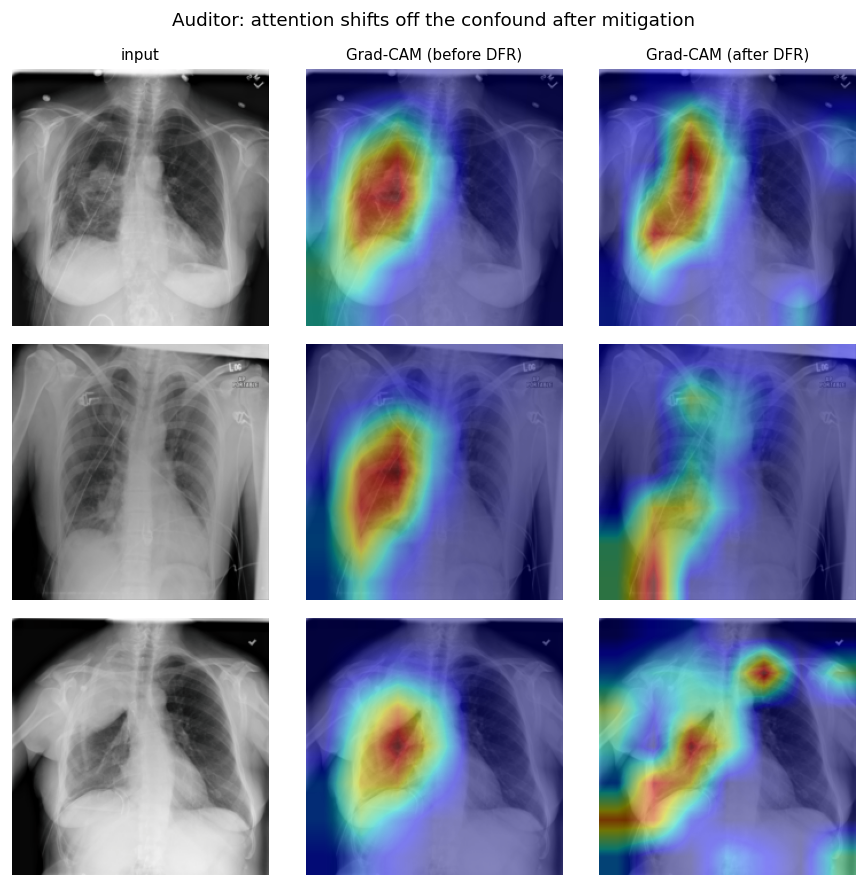
\includegraphics[width=0.9\textwidth]{figures/auditor_before_after_tube.png}
\caption{Before/after Grad-CAM on the real tube model, produced by a single auditor command (detect$\rightarrow$mitigate). After DFR last-layer retraining, attention broadens away from the confound-associated region while in-distribution accuracy is preserved (0.96$\rightarrow$0.97 on this single demo run) and worst-group accuracy rises.}
\label{fig:before_after}
\end{figure*}

The synthetic tag tells the cautionary half of the story: the gap closes (0.44 $\rightarrow$ 0.02) but in-distribution accuracy falls 0.94 $\rightarrow$ 0.62. A linear probe run specifically to falsify the tempting ``the backbone is hollow'' reading measured probe AUC \textbf{0.690} --- above chance (0.50), below the clean baseline (0.845). Shortcut reliance \textbf{degrades but does not eliminate} core-feature learning, and the degradation is strength-dependent.

Cross-site, a real gap exists and is not explained by the shortcut. NIH reference AUC \textbf{0.842} falls to PadChest \textbf{0.650}, a drop of \textbf{0.192} (95\% CI \textbf{[0.159, 0.225]}, stratified bootstrap, 2,000 resamples over the exact test images), matching the magnitude reported by Zech et al.\ \cite{zech2018} --- a robust effect, not a borderline one. Supervised target adaptation recovers \textbf{$+0.082$} --- but that is last-layer fitting on \emph{labeled} PadChest and would help absent any shortcut, so it licenses no mitigation claim. The honest test, zero-shot source-DFR with no target labels touched, returns \textbf{$+0.005$} (95\% CI \textbf{[$-0.018$, $+0.028$]}, same bootstrap procedure). The interval excludes a large recovery and includes zero, so the point estimate is not evidence of a real effect --- but the interval is also wide enough that it does not tightly rule out a small-to-moderate one (up to roughly $+0.03$ AUC): this is an \textbf{underpowered null}, not a \emph{tight} one, and we report it as such rather than as definitive proof that reducing a known real source-side shortcut cannot improve cross-site transfer. The 0.192 drop is distribution shift whose cause this design cannot identify; shortcuts are one unproven candidate among scanner, population, label-pipeline, residual-intensity, and subset-composition differences.

\subsection{Mechanism --- Why Naming Breaks}
\label{sec:mechanism}
V4a and V4b are two points, not a mechanism. Two follow-up experiments ask \emph{why} naming breaks: whether fabrication is driven by the confound's \textbf{visibility}, and whether it is grounded in the image at all.

\subsubsection{Experiment 1 --- the difficulty curve is a recall cliff, not a hallucination cliff}
The intuitive hypothesis is that fabrication rises as the confound gets fainter. We tested it directly by sweeping the synthetic tag's opacity across $\{0.25, 0.5, 0.75, 1.0\}$ and re-scoring both models with the unchanged pipeline ($n = 200$ crops per cell, 100 positive + 100 control), shown in Table~\ref{tab:difficulty}.

\begin{table}[!t]
\caption{Difficulty curve: sweeping synthetic-tag opacity. Reducing visibility produces a recall cliff while control-hallucination stays flat.}
\label{tab:difficulty}
\centering
\begin{tabular}{llccc}
\toprule
\textbf{opacity} & \textbf{model} & \textbf{precision} & \textbf{recall} & \textbf{control-hall.} \\
\midrule
0.25 & scout   & 0.600 & 0.030 & 0.020 \\
0.25 & pixtral & 0.420 & 0.210 & 0.290 \\
0.50 & scout   & 0.963 & 0.520 & 0.020 \\
0.50 & pixtral & 0.588 & 0.400 & 0.280 \\
0.75 & scout   & 0.978 & 0.900 & 0.020 \\
0.75 & pixtral & 0.556 & 0.400 & 0.320 \\
1.00 & scout   & 0.978 & 0.900 & 0.020 \\
1.00 & pixtral & 0.626 & 0.520 & 0.310 \\
\bottomrule
\end{tabular}
\end{table}

Reducing visibility produces a \textbf{recall cliff} --- Scout's recall collapses 0.90 $\rightarrow$ 0.52 $\rightarrow$ 0.03 between opacity 0.75, 0.5 and 0.25 --- while \textbf{control-hallucination stays flat}: $\sim$0.02 for Scout and $\sim$0.28--0.32 for Pixtral across \emph{every} opacity level. Faintness makes the model miss the confound; it does not make the model invent one.

This \textbf{rules out visibility as the bridge} from V4a's 0.02 hallucination to V4b's 0.50--0.83. Whatever separates the synthetic tag from the real tube, it is not how hard the confound is to see. The revised working hypothesis is that fabrication tracks the \textbf{anatomical plausibility of the confound category}: a synthetic tag is never mistakable for anatomy at any opacity --- it is either seen or not, with no ambiguous middle --- whereas a real device sits inside a space of plausible near-misses (other lines, catheters, vessels, fissures, rib edges) that a VLM's medical-image priors can generate confident boilerplate about.

\subsubsection{Experiment 2 --- fabrication is grounded, not blind recitation}
The competing explanation is that the VLM is not reading the image at all --- a live concern, since Lotfinia et al.\ (arXiv:2606.17710) \cite{lotfinia2026} show VLMs can answer chest-radiograph questions from language priors without attending to the image. If V4b's descriptions were prior-emission independent of pixels, the auditor's naming step would be meaningless even where it scores well.

We tested this with three per-crop conditions scored against each model's own unmodified-crop baseline description: occlude the \textbf{relevant} region, occlude an equal-area \textbf{irrelevant} region, or \textbf{swap} in a different same-kind crop. Verdict changes are broken down by direction, because a combined ``changed'' rate conflates opposite outcomes: \textbf{pos$\rightarrow$neg} (named at baseline, not named after) is consistent with grounding; \textbf{neg$\rightarrow$pos} (a \emph{new} device named after the edit) is fabrication merely relocated. All 12 cells are complete at $n = 100$ (Table~\ref{tab:grounding}).

\begin{table}[!t]
\caption{Grounding experiment: verdict changes by direction, per dataset/condition/model, at $n = 100$.}
\label{tab:grounding}
\centering
\footnotesize
\begin{tabular}{lllcccc}
\toprule
\textbf{dataset} & \textbf{condition} & \textbf{model} & \textbf{pos$\rightarrow$neg} & \textbf{neg$\rightarrow$pos} & \textbf{unch.} & \textbf{chg rate} \\
\midrule
v4a & relevant   & scout   & 19 & 5  & 76 & 0.24 \\
v4a & relevant   & pixtral & 25 & 22 & 53 & 0.47 \\
v4a & irrelevant & scout   & 16 & 5  & 79 & 0.21 \\
v4a & irrelevant & pixtral & 27 & 24 & 49 & 0.51 \\
v4a & swap       & scout   & 8  & 8  & 84 & 0.16 \\
v4a & swap       & pixtral & 27 & 23 & 50 & 0.50 \\
v4b & relevant   & scout   & 61 & 1  & 38 & 0.62 \\
v4b & relevant   & pixtral & 66 & 5  & 29 & 0.71 \\
v4b & irrelevant & scout   & 30 & 4  & 66 & 0.34 \\
v4b & irrelevant & pixtral & 13 & 2  & 85 & 0.15 \\
v4b & swap       & scout   & 20 & 21 & 59 & 0.41 \\
v4b & swap       & pixtral & 17 & 17 & 66 & 0.34 \\
\bottomrule
\end{tabular}
\end{table}

A measurement artifact requires that most of this table be read with care. The flat gray fill used to occlude the tag is \emph{itself} routinely described by the VLM as ``a gray rectangular object\ldots artificial and not part of the patient's anatomy\ldots a label or marker'' --- language that trips the exact \texttt{names\_confound} rule the tag was designed to trigger. Spot-checking confirms it: \textbf{76 of 100} Scout descriptions under V4a \emph{relevant} occlusion still flag positive, matching the \texttt{unchanged} count, and reading them shows the model is describing the \textbf{occlusion patch itself}, not residual tag content. Consequently \textbf{V4a's \texttt{relevant} numbers understate true grounding}, and the V4a-vs-V4b comparison is invalid for this question --- the measurement is biased toward \texttt{unchanged} for V4a in a way it is not for V4b.

\textbf{The evidence that carries the conclusion is the V4b-internal contrast.} V4b's matcher (\texttt{names\_tube}) requires device-specific vocabulary --- which a flat gray rectangle does not resemble the way it resembles a generic ``artificial marker'' --- so its susceptibility to the artifact is far lower (only 38 of 100 Scout descriptions stay unchanged-positive under V4b relevant occlusion, vs V4a's 76). Within V4b, both conditions use the same matcher on the same dataset, differing only in \emph{where} the occluder lands:
\begin{itemize}
\item Occluding the \textbf{tube region} drops device-naming: pos$\rightarrow$neg \textbf{61/100} (Scout), \textbf{66/100} (Pixtral).
\item Occluding an equal-area \textbf{irrelevant} region drops it far less: \textbf{30/100} (Scout), \textbf{13/100} (Pixtral).
\end{itemize}

Device-naming tracks the tube pixels. ``V4b fabrication is pure image-independent prior-emission'' is not supported. The reconciled mechanism, read against the 50--83\% control-hallucination on clean crops: the VLM carries a strong \textbf{device-present prior} \emph{and} grounds it on the salient region --- correctly reading a real tube when one is present, and \textbf{over-reading ambiguous normal anatomy as a device} when none is. This is prior-driven over-reading of an ambiguous salient region: neither blind recitation nor clean perception, and it coheres with Experiment 1's finding that plausibility, not visibility, is the operative axis. (Supporting but not load-bearing: V4b's swap condition is near-symmetric --- 20/21 Scout, 17/17 Pixtral --- and \texttt{text-identical-rate} was 0.0 in every cell, so verbatim recitation is not the failure mode. A texture-matched occluder should replace the flat gray fill in replication, to clean the V4a arm.)

\subsection{Specialist VLM}
\label{sec:specialist}
The V4b mechanism above was established for general-purpose VLMs only, leaving one escape hatch: maybe a radiology-fine-tuned VLM, carrying a device vocabulary the general models lack, would clear the gate the general models failed. It does not --- but the \emph{way} it fails is the result. Six additional models were run on the \textbf{identical} V4a/V4b crops and the same blind prompt (byte-verified against the general arm's), scored with the existing project matchers. Three are reportable; \textbf{three are excluded as harness output bugs, not model results}, and their zeros are not findings: \textbf{phi3.5-vision} returned an empty string on all 200 crops in both arms; \textbf{qwen2.5-vl-3b} produced the refusal ``no image attached'' on 164/200 V4a crops --- the image never reached the model; \textbf{MedGemma} returned 400 blank responses from a quantized-vision-tower bug, diagnosed separately with a re-run pending. Reporting any of these as a naming failure would be a fabrication of the opposite kind. \emph{Three models reported; three excluded for harness output bugs.}

The three reportable models --- qwen2.5-vl-7b, CheXagent-2-3B, and chexagent-8b --- split cleanly on a single axis: whether they \textbf{over-name} or \textbf{under-name} the device. Both failure modes clear neither V4b gate, but for opposite reasons, and the split is the contribution.

\textbf{General VLMs over-name, and it is not a small-model artifact.} The V4b fabrication that triggered the pivot was a general-VLM behavior: on tube-free controls, Llama-4-Scout fabricates a device on \textbf{0.55} of clean crops (95\% bootstrap CI [0.45, 0.65]) and Pixtral-12B on \textbf{0.83} ([0.75, 0.90]). qwen2.5-vl-7b --- a \emph{larger} general VLM, and the only new model with non-trivial signal (V4a precision \textbf{0.63} / recall \textbf{0.33}) --- over-names just as hard: its V4b control-hallucination is \textbf{0.74}. Over-naming is therefore not an artifact of the 12B-and-under general models that first exhibited it; it persists at 7B on a fresh model family, at a rate that still fails the $<$0.10 control-hallucination bar sevenfold.

\textbf{The medical specialist under-names --- a structural zero.} CheXagent-2-3B does not answer in free text; it emits its own referring-expression grounding tokens (\texttt{<|ref|> foreign object <|/ref|> <|box|>\ldots<|/box|>}). Scored with a grounding-aware matcher that holds it to the \emph{same} genericness bar as the general models, it clears V4a's precision handsomely (precision \textbf{0.9663}, recall \textbf{0.86}, control-hallucination \textbf{0.03}) --- near the gate and far below the fabrication bar. On V4b it scores exactly \textbf{0.0 / 0.0 / 0.0}. This is not a perception failure: CheXagent produced a grounded label on \textbf{100/100} V4b tube-positive crops. It is a \emph{taxonomy} failure. Its entire observed grounding vocabulary is $\{$foreign object, diaphragm, other lesion, artificial object, aortic enlargement, mediastinal$\}$ --- \textbf{no device-specific class exists anywhere in its output space}: nothing that says tube, catheter, line, drain, or wire, in either dataset. The specialist can localize the tube and cannot \emph{name} it, because ``name it as a device'' is not an option its taxonomy affords. Where the general VLMs fail V4b by saying too much on clean crops, the specialist fails by having no word for the thing it is grounding on.

\textbf{Under-naming survives a 3B$\rightarrow$8B scale-up.} chexagent-8b, the larger sibling, answers in free-text radiology-report prose rather than grounding tokens, and scores \textbf{0.0 / 0.0 / 0.0} on both arms: its prose never reaches the device vocabulary the matchers key on, with no compensating control false positives. The under-naming ceiling is thus not a 3B capacity limit --- it clears a 3B$\rightarrow$8B scale-up unchanged --- but a property of how the specialist's output space was designed. Naming a device is a vocabulary-design decision made upstream of scale.

\textbf{One caution against an over-clean reading.} ``Specialist under-names, general over-names'' is the axis, but it is not the \emph{only} axis, and the general models are not uniformly safe wherever the specialist is silent. Even on the easy \textbf{synthetic} V4a controls, fabrication is model-dependent: Scout hallucinates on \textbf{0.02} of clean crops ([0.00, 0.05]) but Pixtral on \textbf{0.31} ([0.22, 0.40]) --- a per-model fabrication \emph{floor} that has nothing to do with domain specialization. The clean ``synthetic naming is safe'' story is Scout-specific; another general VLM fabricates on a third of the same easy controls. The auditor's reliability therefore turns on the specific model on both axes at once --- how much it over-names on clean crops \emph{and} whether its vocabulary can name the target at all --- and neither axis is settled by the general-vs-specialist label alone.

\subsection{Supporting Evidence and Robustness}
Five VLM-independent investigations probe the robustness of the results above. None is a headline; each either strengthens a claim by an independent route or bounds an alternative explanation.

\textbf{The tube shortcut is severity-invariant (underpowered).} Stratifying the 94 overlapping pneumothorax-positive test images at the median bounding-box area and balancing groups within each tier, accuracy is perfect whenever a tube is present, at \emph{any} lesion size, and collapses when it is absent, at \emph{any} lesion size (low-severity gap 0.400 at $n$=20; high-severity gap 0.4375 at $n$=16). The gap is large in both tiers, which rules out a pure disease-burden proxy, but at $n$=16--20/group it is underpowered to distinguish true invariance from a real severity effect, so the invariance claim is withdrawn; what stands is that even low-severity cases show a large gap --- the shortcut is \textbf{device-keyed, not disease-burden-keyed}.

\textbf{The DFR result is a floor, not a ceiling.} A canonical DFR variant (regularization $C$ tuned by 5-fold CV, weights averaged over 10 balanced draws) strictly dominates single-draw DFR on the real tube (worst-group 0.84$\rightarrow$0.93, ID 0.965$\rightarrow$0.998, gap 0.12$\rightarrow$0.07), confirming the reported result is not a lucky hyperparameter. On the synthetic tag it recovers some ID accuracy (0.594$\rightarrow$0.687) but remains far below the 0.94 baseline; the tag ``closing'' the gap is partly an artifact of the symmetric tagged/untagged validation construction, documented as an anomaly, and the tube result is the one we defend.

\textbf{Site identity is redundantly encoded (a stronger restatement of the V6 null).} A hospital detector separates NIH from PadChest from the frozen penultimate features at AUC \textbf{0.9993}, yet projecting that site direction out and re-scoring the frozen disease head leaves disease AUC \textbf{unchanged (0.6436 $\rightarrow$ 0.6436, $\Delta$ 0.000)}. A fresh probe on the projected features still reaches AUC 0.9990 --- a rank-1 projection removes essentially none of the site signal, correcting an earlier over-claim: site information is redundantly encoded across many directions. The disease-AUC null stands regardless, since it is measured on the frozen head.

\textbf{Label-free OOD attribution: the synthetic-vs-real asymmetry.} Generalizing the zero-shot source-DFR test to the synthetic tag, source-side tag mitigation does not merely fail to transfer --- it \emph{actively hurts} transfer ($-0.083$ on PadChest, vs the tube's $+0.005$ null). A \emph{pure} synthetic shortcut at $p$=0.95 is a near-total representation override; the tube model retains genuine disease signal alongside its shortcut while the tag model largely stops learning the disease. Synthetic confounds prove the \emph{method} but systematically overstate the \emph{severity} of the phenomenon relative to real ones, and should not be extrapolated to real shortcuts without the real-arm check.

\textbf{Where reliance turns on: the correlation sweep.} Sweeping correlation strength \emph{p} at \textbf{one training seed per point} (a limitation carried through to the Limitations section), the reliance gap rises monotonically \textbf{across these five single-seed runs} --- 0.000 ($p$=.6) $\rightarrow$ 0.010 $\rightarrow$ 0.075 $\rightarrow$ 0.294 $\rightarrow$ 0.440 ($p$=.95) --- a trend, not yet a seed-replicated result at the training level, with an \textbf{onset threshold}: below $p \approx 0.7$ the correlation is too weak to exploit and the model learns real signal (test AUC $\approx$ 0.83). DFR's in-distribution cost is correspondingly strength-dependent, negligible where there is no shortcut and large where it was allowed to dominate. The DFR-recovery step was re-run at 3 seeds on the frozen per-\emph{p} checkpoints; every single-seed value falls within roughly one standard deviation of those means, so the sweep's conclusions do not hinge on the seed (the \emph{training}-seed variance of the gaps themselves is not claimed).

\textbf{A fifth investigation, reported as blocked.} Severity-\textbf{aware} mitigation was not run: severity labels exist only for the 94-image test split, and no proxy was fabricated. It is reported as blocked rather than omitted.

% =====================================================================
\section{Discussion}
The paper's spine is a boundary: blind, general-purpose VLM naming works where a shortcut is unmistakable and fails --- by fabrication --- where a shortcut is a plausible member of a familiar category. The two mechanism experiments locate \emph{which} axis the boundary runs along. It is not visibility: faintness produces a recall cliff, not a hallucination cliff (Experiment 1). It is plausibility. A synthetic corner tag is never mistakable for anatomy at any opacity, so the model either sees it or does not; a chest tube lives among lines, catheters, vessels, fissures, and rib edges that a device-primed VLM can write confident boilerplate about. Experiment 2 then rules out the deflationary reading that the VLM ignores the image: device-naming tracks the tube pixels (occluding the tube drops naming roughly twice as much as occluding an equal-area irrelevant region). The failure is therefore neither blind recitation nor clean perception --- it is \textbf{prior-driven over-reading of an ambiguous salient region}.

We frame the failure as an \textbf{over-name / under-name axis}, because the two directions carry different costs for an auditor. Under-naming (a miss) degrades gracefully --- Experiment 1 shows that as the confound fades the model simply stops naming it, and the recall bar is set below precision precisely to tolerate this. Over-naming (fabrication) is the dangerous direction: a tool that invents a chest tube on a clean radiograph will send a clinician chasing a shortcut that is not there, and at 55--83\% on clean crops it would do so on a majority of images. This is why the design made control-hallucination a \emph{gate} rather than a reported statistic, and why the honest verdict is that off-the-shelf general VLMs are not safe as blind auditors of clean images without such a gate. That the boundary is \textbf{per-model} rather than a flat clean split (Figure~\ref{fig:naming_boundary}: Scout fabricates on 2\% of synthetic controls but Pixtral on 31\%) sharpens rather than softens the conclusion: even in the ``easy'' synthetic setting, one of two general models already fails the gate.

What survives the naming failure matters for how the contribution should be read. The mitigation result is real, defensible, and --- by construction --- independent of the broken naming step: no method in the mitigation path imports the VLM module, so the naming-off ablation is not a separate experiment but a property of the code. DFR recovers worst-group accuracy on the real tube from 0.67 to 0.79 (3-seed mean) with in-distribution accuracy preserved and no target-distribution labels, and two independent methods agree well outside seed variance. We are deliberate about the headline number: 0.79 is the 3-seed mean; the single-draw 0.83 appears only when explicitly labeled as such, because reporting the luckier draw as the result would be the same over-claiming the paper's method is designed to catch. The synthetic tag supplies the cautionary companion --- a pure shortcut at $p$=0.95 so thoroughly overrides the representation that removing it leaves too little disease signal behind, which is exactly why synthetic confounds prove the \emph{method} but overstate the \emph{phenomenon}.

The cross-site result is where we most resist the tempting story. There is a real 0.192 US-to-Spain AUC drop, Zech-magnitude, and it would be easy to present the loop as ``validated cross-site.'' It is not. The supervised recovery ($+0.082$) uses PadChest labels and would help with no shortcut present; the honest zero-shot source-DFR test --- reduce the \emph{known} tube shortcut on NIH only, touch no target labels --- returns $+0.005$ (95\% CI [$-0.018$, $+0.028$]): a point estimate indistinguishable from zero, on an interval too wide to also rule out a small-to-moderate effect. Reducing a known source shortcut did not measurably narrow the cross-site gap in this test, so the gap is distribution shift this design cannot attribute to the shortcut --- while acknowledging the test's power to detect a modest effect, had one existed, was limited. The representation-level controls corroborate rather than rescue this: site identity is almost perfectly decodable (AUC 0.9993) yet the frozen disease head does not read it ($\Delta$ 0.000 after projecting site out), so the two mechanisms one reaches for first --- a head riding a site signal, and a covariate shift correctable by label-free adaptation --- are both bounded near zero, leaving most of the gap genuinely unattributed. The clinically load-bearing consequence is that ``fix the known shortcuts'' is \emph{not} sufficient due diligence before cross-site deployment.

Finally, honest scope. This is one pathology (pneumothorax), one primary corpus (NIH) with one second site (PadChest), one real device confound (chest tube) with non-expert labels, and general (not specialist) VLMs. The two mechanism experiments bound the boundary on the visibility and image-grounding axes but do not map it along the plausibility axis the mechanism implicates --- we know naming works on an unmistakable marker and fails on a subtle device, not where in between it turns over. The pre-registered stopping rule governed the gate decision itself --- a V4b failure after a V4a pass triggered an immediate, reported pivot rather than iteration on that decision --- but it did not foreclose a cheap follow-up ablation (abstention prompting), which was designed and coded but not executed before this writeup (see Limitations). The boundary is therefore \emph{characterized}, not \emph{mapped}, partly by design and partly because that follow-up remains unrun.

% =====================================================================
\section{Limitations}
\textbf{Single pathology, single primary corpus.} Every result concerns pneumothorax on NIH ChestX-ray14 and its cross-site evaluation on PadChest. The mechanism proposed in Section~\ref{sec:mechanism} --- fabrication driven by the anatomical plausibility of the confound category --- predicts that other device-adjacent pathologies would behave similarly, but this is a prediction, not a measurement.

\textbf{Non-expert ground truth for the real confound.} NEATX's chest-drain annotations come from two data-science students, not radiologists, with ``moderate to almost perfect'' agreement against expert labels reported in the source paper. This is adequate for inducing a training-time enrichment signal and defining a mitigation target, but it is a noisier ground truth than a radiologist-drawn segmentation --- and it bears most heavily on exactly the number the paper turns on: V4b's precision and recall are scored \emph{against these labels}. A radiologist-grade corpus (e.g.\ CANDID-PTX, whose access requires an ethics-training pathway we did not complete in time) would be the appropriate ground truth for re-scoring the naming gate specifically.

\textbf{The auditor's own VLM component was not tested for pure image-independence in V4a.} Lotfinia et al.\ (arXiv:2606.17710) \cite{lotfinia2026} show VLMs can answer CXR questions from language priors without attending to the image. Experiment 2 addresses this and does \emph{not} support blind recitation as the explanation of V4b (device-naming tracks the tube pixels), but a clean counterfactual-image test on V4a specifically --- free of the flat-gray-occluder artifact documented in Section~\ref{sec:mechanism} --- remains the most direct follow-up to strengthen V4a's interpretation.

\textbf{Two-site validation; V6 causal attribution narrowed but not closed.} Two sites are two points, not a trend. The cross-site drop (0.192) is real and Zech-magnitude, and the robustness controls rule out two candidate mechanisms --- a disease head riding a decodable site signal ($\Delta$ 0.000) and label-free covariate shift correctable by standard test-time adaptation (BN-adaptation $-0.004$; TENT $-0.122$, actively harmful). But most of the gap remains genuine, unattributed distribution shift. Candidate causes this design cannot separate include scanner and acquisition differences, population differences, the two datasets' different label-generation pipelines (NIH's NLP-only labeler vs.\ PadChest's NLP-plus-manual process), residual intensity artifacts despite the 8-bit fix, and the composition of the 573-positive / 7,000-negative working subset. Label semantics are known to differ in a direction that can inflate the gap --- among PadChest's 573 pneumothorax-positives, only 15.7\% carry pneumothorax as the sole finding, and the most common co-finding is a chest drain tube (109 cases, $\approx$19\%) --- but the working-subset CSV lacks the fields needed to quantify this, so it is bounded qualitatively. A third site would turn two points into a trend; the design accommodates one without rework, but we did not run it.

\textbf{Single-GPU scale; single-seed sweep.} All training ran on one consumer GPU (RTX 3050, 6GB), which shaped batch size (16, after an OOM at 32), resolution (224px, standard for this literature), and the decision to work with subsets (most visibly the 7,572-image PadChest working set against the full release's 160,861). The correlation sweep carries one \emph{training} seed per point for the same reason; its trend (monotone reliance growth) is clear, but individual point values could shift under a different seed. The 3-seed baseline table is the result we defend most strongly on variance grounds. Nothing measured appears to depend on the hardware in a way that would not reproduce at scale, but larger-scale replication was out of reach and is not claimed.

\textbf{The difficulty boundary is bounded on one axis, unmapped on the others.} Experiment 1 rules out visibility as the axis along which naming degrades into fabrication, and the multi-VLM replication closes the ``a different model would fix it'' escape hatch for general-purpose VLMs (55\% and 83\% fabrication on clean crops). What remains open is where between an unambiguous synthetic marker and a subtle real device the boundary sits along the \emph{plausibility} axis, and whether prompt design, crop resolution, or abstention/confidence mechanisms shift it. An abstention-prompt ablation targeting exactly this --- suppress a device claim unless the model is confident it is not normal anatomy --- was designed and implemented (\texttt{ABSTENTION\_PROMPT}, \texttt{names\_tube\_abstention()}, unit-tested) as part of the multi-VLM study, but was not executed against the V4b crops before this writeup; we report it as built-but-unrun rather than as a considered decision not to attempt a rescue, since the design documents show the intent was to run it. Whether abstention would have moved V4b's control-hallucination is therefore an open, cheaply answerable question (the crops, prompt, and scorer already exist) rather than one closed by a stopping rule. The pre-registered pivot rule did govern the \emph{headline} gate decision --- V4b's FAIL was reported and acted on immediately rather than iterated around. The specialist-VLM arm addresses the narrower question of whether radiology fine-tuning moves the boundary at all.

\textbf{Interpretive claims corrected mid-project.} Two claims were written before the control that tests them existed, and both were withdrawn once it was run: ``the pure-shortcut backbone is hollow'' (falsified by the linear probe: AUC 0.690, above chance 0.50) and ``mitigation validated across three settings'' (falsified by the zero-shot source-DFR null: $+0.005$, after the $+0.082$ ``recovery'' was correctly re-identified as supervised target adaptation). We report both, because the failure mode they share --- asserting an interpretation the experiment does not license --- is the same one this paper's method is designed to catch in a classifier, and there is no principled reason to exempt the authors from it.

% =====================================================================
\section{Conclusion}
We set out to build an auditor that detects, names, and mitigates a spurious shortcut in a chest X-ray classifier, and we ran it under a validation-gated discipline that let each stage's claim stand or fall on a pre-registered threshold. Detection, localization, and mitigation transfer from a synthetic confound to a real chest-tube confound: reliance is measurable, attributable, and reducible --- worst-group accuracy on untreated (tube-free) pneumothorax rises from 0.67 to 0.79 with no target labels, on a step that provably never touches the VLM. The naming stage does not transfer. Blind, general-purpose VLM naming passes at near-ceiling on an unmistakable synthetic marker and fails on the real device by \emph{fabrication}, inventing chest tubes and catheters on a majority of clean radiographs --- a cross-model failure, corroborated by independent benchmarks, that our control-hallucination gate was built to catch and did. And the real cross-site drop we measured is distribution shift we could not attribute to the shortcut, not a mitigation success.

The contribution we stand behind is therefore not ``an auditor that names shortcuts,'' but a mapped boundary of where that ambition currently breaks and a defensible mitigation result that survives the break. Blind VLM naming is a bounded capability --- trustworthy for salient, unambiguous shortcuts, unsafe as a blind auditor of clean images without a false-alarm gate. The most useful thing a capstone can do with a failed critical gate is report it precisely, characterize why it fails, and show what still works around it. That is what this paper does: an honest negative result on generative-model-free shortcut naming, wrapped in a mitigation and cross-site study that neither overstates the recovery nor hides the failure. The natural next steps --- a radiologist-grade real-confound corpus for re-scoring the gate, a specialist-VLM arm to test whether radiology fine-tuning moves the boundary, and a third site to turn two cross-site points into a trend --- are all accommodated by the confound-agnostic design without rework.

% =====================================================================
\section*{Acknowledgment}
% TODO: acknowledgements — none asserted by the source draft. Add data-use
% credits (NIH ChestX-ray14, PadChest, NEATX) and any funding here.

% =====================================================================
% References. Uses the IEEE Access BibTeX style shipped with the template.
% These three appear in the source draft's References list but are not cited
% inline in its body; \nocite keeps them in the compiled bibliography so the
% reference list matches the source draft exactly.
\nocite{dfr_multilayer,sourget2025,rafferty2026}

\bibliographystyle{ieeeaccess}
\bibliography{references}

% -----------------------------------------------------------------
% Author biography (IEEE Access requires one per author on acceptance).
% TODO: add \begin{IEEEbiography}...\end{IEEEbiography} block(s) once the
% author is de-anonymized. The template's \EOD macro may follow the last
% biography; omitted here because no biography is present.
% -----------------------------------------------------------------

\end{document}
